\chapter{Análisis y diseño}

\section{Análisis de requisitos}

Todo software se desarrolla para cubrir una necesidad, por lo que en este apartado vamos a describir los requisitos que se 
estiman necesarios para cubrir los objetivos propuestos.

\subsection{Descripción de los actores}

Los actores implicados serán dos: el \textbf{desarrollador} y el \textbf{usuario}.

\bigskip
El \textbf{desarrollador} será el encargado de solucionar los problemas de visualización de los datos en la plataforma, además de 
portar el desarrollo actual de la plataforma a un entorno de desarrollo continuo. También asumirá la administración de la 
plataforma ya que este tipo de rol está muy integrado con las labores de despliegue en el desarrollo continuo.

\bigskip
El \textbf{usuario} de la aplicación será cualquier persona que tenga interés por conocer datos internos de la Universidad de Granada 
fácilmente. El usuario no pertenece a ningún público objetivo concreto, por lo que no se tiene que considerar que tenga una
experiencia previa en navegador por sitios web.

\subsection{Requisitos Funcionales}

Los requisitos funcionales son las características que tiene que implementar el sistema para cubrir todas las necesidades de 
los distintos usuarios.

\bigskip
Al usuario lo único que le interesa es ver una página web estática con la información que desea 
consultar, para ello el desarrollador deberá hacer que sea posible que se generen siempre las tablas con los elementos de 
información. 

\bigskip
Por otra parte, el desarrollador quiere integrar el sistema en un desarrollo continuo, por lo que añadirá tests 
unitarios, test de cobertura, integración continua, despliegue automático y aprovisionamiento con tal fin.

\begin{itemize}
  \item \textbf{RF-1.} Acceso a la información:
    \begin{itemize}
    \item \textbf{RF-1.1.} Generar tablas con elementos de información.
    \item \textbf{RF-2.2.} Consultar tablas con elementos de información.
    \end{itemize}
\end{itemize}

\begin{itemize}
  \item \textbf{RF-2.} Introducción del desarrollo continuo:
  \begin{itemize}
    \item \textbf{RF-2.1.} Realizar tests unitarios.
    \item \textbf{RF-2.2.} Realizar test de cobertura.
    \item \textbf{RF-2.2.} Realizar integración continua.
    \item \textbf{RF-2.3.} Realizar despliegue automático.
    \item \textbf{RF-2.4.} Realizar aprovisionamiento.
    \end{itemize}
\end{itemize}

\subsection{Requisitos no Funcionales}

Los requisitos no funcionales son las características propias del desarrollo, pero que no tienen que estar relacionadas con su 
funcionalidad.

\begin{itemize}
  \item \textbf{RN-1.} Toda la programación del portal se hará en Node.js y los módulos que se usen deben ser instalables a 
  través de su gestor de paquetes NPM.
  \item \textbf{RN-2.} El portal se iniciará y se detendrá mediante scripts lanzados con NPM.
  \item \textbf{RN-3.} Para iniciar la ejecución del portal es necesario que reciba el puerto de escucha del servidor y la 
  dirección de acceso.
  \item \textbf{RN-4.} Todos los módulos se ejecutarán desde scripts lanzamos con NPM.
  \item \textbf{RN-5.} Los tests unitarios se realizarán en base a comportamientos esperados y valores de estados
  recibidos como contestación a las peticiones que se realicen al portal.
  \item \textbf{RN-6.} Los tests unitarios tienen que recibir las páginas del portal para ejecutarse.
  \item \textbf{RN-7.} El test de cobertura tiene que tener una automatización integrable con los tests unitarios. 
  \item \textbf{RN-8.} La integración continua se ejecutará automáticamente con cada cambio que se haga en la programación
  del portal.
  \item \textbf{RN-9.} El despliegue automático se realizará mediante conexiones SSH.
  \item \textbf{RN-10.} Tanto para el despliegue automático como para el aprovisionamiento es necesario indicar el usuario que
  lo realiza y el destino en el que se realiza.
\end{itemize}

\subsection{Requisitos de Información}

Los requisitos de información se refieren a la información que es necesaria almacenar en el sistema. La única información 
relevante que se va a almacenar son los datos descriptivos y de enlace de cada uno de los elementos del portal OpenData UGR 
que se van a mostrar en UGR Transparente.

\begin{itemize}
  \item \textbf{RI-1.} Datos abiertos.
  \begin{itemize}
    \item Información sobre cada uno de los elementos que se van a mostrar en el portal de transparencia como datos abiertos.
    \item Contenido: nombre, categoría, conjunto de datos, enlace a OpenData UGR, enlace al recurso.
  \end{itemize}
\end{itemize}

\section{Modelos de casos de uso}

Aunque ya se ha indicado que la parte funcional ya se encuentra implementada de forma previa a este proyecto, se van a incluir
unos modelos de caso de uso simples para dar un visión más clara del funcionamiento general de la plataforma UGR Transparente.

\subsection{Descripción básica de actores}

\begin{itemize}
  \item \textbf{Ac-1.} Usuario
  \begin{itemize}
   \item Descripción: Persona que usa la plataforma que consulta datos.
   \item Características: Es el usuario común que accederá a la página.
   \item Relaciones: Ninguna.
   \item Atributos: Ninguno.
   \item Comentarios: El usuario no es necesario que tenga ningún conocimiento previo al uso de la plataforma, simplemente
   accederá y consultará los datos que sean de su interes.
  \end{itemize}
  
  \item \textbf{Ac-1.} Desarrollador
  \begin{itemize}
   \item Descripción: Encargado de añadir los elementos de información a la plataforma.
   \item Características: Su trabajo está en el lado del servidor que genera la página, nunca trabaja desde el lado del cliente.
   \item Relaciones: Ninguna.
   \item Atributos: Ninguno.
   \item Comentarios: Es el encargado de desarrollar las funcionalidades del portal, entre ellas añadir nuevos elementos de
   información.
  \end{itemize}
\end{itemize}

\subsection{Descripción casos de uso}

\begin{itemize}
 \item \textbf{CU-1.} Añadir elemento
 \begin{itemize}
  \item Actores: Desarrollador
  \item Tipo: Primario, Esencial
  \item Precondición: Ninguna
  \item Postcondición: Nuevos elementos de información serán visualizados en el portal de transparencia
  \item Propósito: Son añadidos nuevos elementos de información al portal de transparencia.
  \item Resumen: Aparecerán nuevos elementos de informaciónen la categória que corresponda, acompañado además de su enlace
  correspondiente al OpenData UGR, un botón para previsualizar la información y otro botón para descargar el elemento.
 \end{itemize}
\end{itemize}

\begin{itemize}
 \item \textbf{CU-2.} Consultar elementos
 \begin{itemize}
  \item Actores: Usuario
  \item Tipo: Primario, esencial
  \item Precondición: Existan elementos de información.
  \item Postcondición: Se muestran los elementos de información de un determinado conjunto de datos.
  \item Propósito: Obtiene los elementos de información de un determinado conjunto de datos.
  \item Resumen: Accediendo a través del panel principal o el buscador se obtiene una tabla con los elementos de información
  de un determinado conjunto de datos.
 \end{itemize}
\end{itemize}

\begin{itemize}
 \item \textbf{CU-3.} Acceder enlace de elemento
 \begin{itemize}
  \item Actores: Usuario
  \item Tipo: Primario, esencial
  \item Precondición: Se hayan generado las tablas con los elementos de información.
  \item Postcondición: 
  \item Propósito: Accede a la información del elemento contenida en OpenData UGR.
  \item Resumen: Cuando se pulsa el enlace, se accede al conjunto de datos que contiene la información del elemento en OpenData
  UGR, presentándolo de distinta forma en función del formato del elemento y dando la opción de descagar ese mismo elemento en 
  un archivo con su formato original.
 \end{itemize}
\end{itemize}

\begin{itemize}
 \item \textbf{CU-4.} Previsualizar elemento de información
 \begin{itemize}
  \item Actores: Usuario
  \item Tipo: Secundario
  \item Precondición: Se hayan generado las tablas con los elementos de información.
  \item Postcondición: 
  \item Propósito: Previsualiza los datos del elemento.
  \item Resumen: Cuando se selecciona el botón de ver un elemento de la tabla se abre una ventana emergente en la que se 
  muestra la información del elemento que se contiene en OpenData UGR.
 \end{itemize}
\end{itemize}

\begin{itemize}
 \item \textbf{CU-5.} Descargar elemento de información
 \begin{itemize}
  \item Actores: Usuario
  \item Tipo: Secundario
  \item Precondición: Se hayan generado las tablas con los elementos de información.
  \item Postcondición: 
  \item Propósito: Descagar el elemento en un archivo con su formato original.
  \item Resumen: Cuando se selecciona el botón de descargar un elemento de la tabla se abre una ventana emergente en la que se
  muestra la información del elemento que se contiene en OpenData UGR.
 \end{itemize}
\end{itemize}

\subsection{Diagramas de casos de uso}

Desde un punto de vista funcional es el usuario el que realiza la mayoria de las acciones del portal, la función del 
desarrollar aunque fundamental, solo es una acción que se realiza en un segundo plano del que no se tiene constancia desde 
fuera.

\begin{figure}[!h]
  \begin{center}
  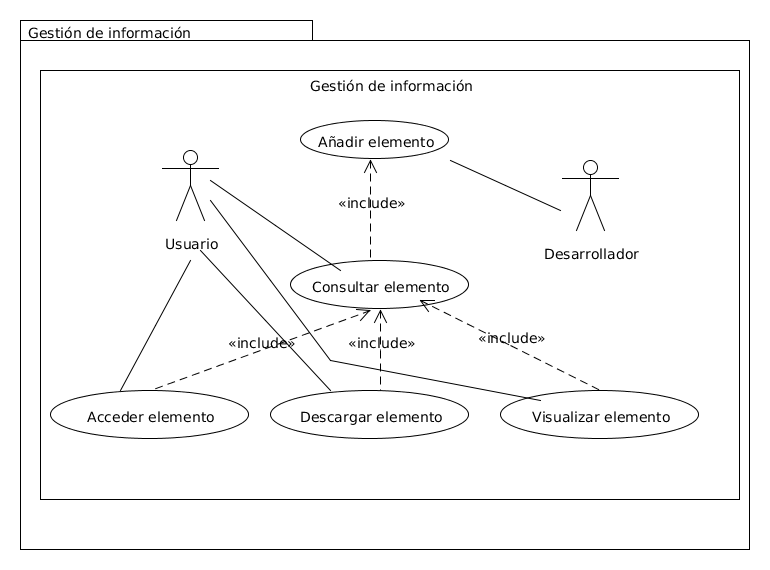
\includegraphics[width=1\textwidth]{imagenes/diagrama_casos_uso.png}
  \caption[Casos de uso]{Diagrama de casos de uso}
  \label{fig:casosUso}
  \end{center}
\end{figure}

